\chapter{What Comes Next}
\label{ch:outlook}

A reader who came to this book from the Bitcoin side brought one question to page one, and it is time to answer it: does the grid save mining, or does mining serve the grid? Nine chapters have said, in effect, both, and the ledger of Chapter~9 priced what serving the grid was worth to one site over five years. This last chapter looks forward through arithmetic the reader can check. Three sums carry the chapter. The first is what happens to the flexibility stack if hashprice keeps falling as future halvings cut the subsidy. The second is the block subsidy set against any path the price of bitcoin can plausibly take. The third is the \glossaryterm{security-budget}{security budget}, what the network pays for the hashes that protect it, and who will pay it when the subsidy is gone. Chapter~9 handed this chapter three things whose rules change after its data ends, and each gets its place: RTC+B, which turned reserves into a priced option; 12CP and the minimum billing demand, which, if adopted as proposed, end the peak layer for new large loads; and hashprice, which rests on a subsidy that halves on a schedule. One convention is fixed here for the whole chapter. Where a dollar figure depends on the price of bitcoin, it uses \$81,273, the last price in the companion repository's daily series, on September 4, 2026; Chapter~4 used the August price of about \$66,000. Every such line scales in proportion, so the reader can rescale it on the day they read, and none of it is a price forecast: Chapter~5 explained why forecasting is not this book's habit. Every prediction here is my reading of those three sums, labeled as such, and you can run them with other numbers in the companion repository. % src: analysis/checks/ch10_subsidy_arithmetic.R console (reference price $81,273 on 2026-09-04, blockchaininfocharts); chapter 4 ($66,180 seven-day mean to 2026-08-21, analysis/data/btc_price_daily.csv); chapter 9 sec:stack-rule (the three hand-offs)

\section{The Cheaper the Hash, the Better the Grid Resource}
\label{sec:outlook-cheaper}

Chapter~9 found that the old machine did most of the site's grid work. The S19j~Pro, with a strike of \$72 in 2025, paused 14~percent of the year and earned nearly three times as much from the strike per megawatt as the S21~XP, whose strike of \$157 sat above almost every price the year produced. % src: chapter 9 sec:stack-strike (paused 14% vs under 3%; per MW-yr 45,983 vs 15,938 = 2.9x)
That asymmetry follows from where any machine's strike sits relative to the power price, and the strike is hashprice times 41,667 divided by efficiency, Chapter~4's identity. Every machine's strike falls with hashprice, and hashprice fell six-fold from 2021 to 2025. So what does the stack of Chapter~9 look like as every machine becomes what the S19j~Pro is today? % src: chapter 4 (the 41,667 identity); chapter 9 sec:stack-site (spliced hashprice $0.310 in 2021 to $0.051 in 2025)

Here, the ``optimal site'' uses the price-response loop and plays the summer window where it pays over the modeled year. The loop acts on past prices; the annual window choice uses the year's results.

\begin{figure}[htbp]
  \centering
  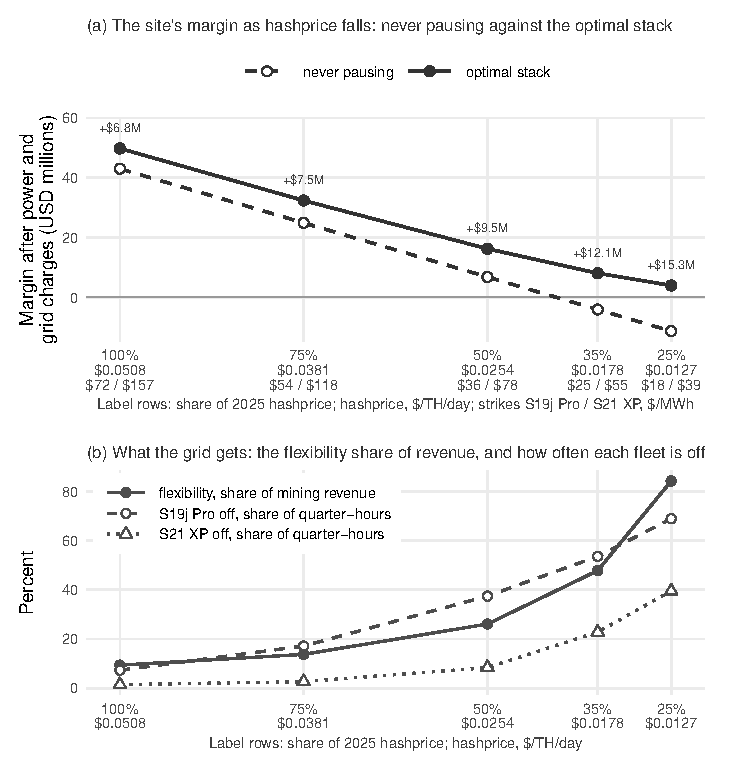
\includegraphics[width=\textwidth]{images/ch10_hashprice_sensitivity}
  \caption{Chapter~9's reference site on 2025 LZ\_WEST prices, with the daily hashprice scaled from 100 to 25~percent of its actual path. (a)~Margin after power and grid charges of the never-pausing site against the optimal stack; the axis carries the share, the hashprice in dollars per terahash-day and the two strikes; the label on each point is the value of flexibility. (b)~Flexibility as a share of mining revenue, and the share of quarter-hours each fleet spends switched off under the optimal stack; with the power target available the site prefers to underclock rather than stop, so the off share sits below the pause share of a plain strike rule. Lagged decisions, measured power curves and 2025 grid charges; the summer window is played where it pays, and reserves are left aside.} % fig-src: analysis/figures/fig_ch10_hashprice_sensitivity.R on analysis/data/ch10_hashprice_sensitivity.csv (ch10_hashprice_sensitivity.R)
  \label{fig:outlook-sensitivity}
\end{figure}

Figure~\ref{fig:outlook-sensitivity} and Table~\ref{tab:outlook-sensitivity} rerun the 2025 ledger with hashprice scaled down, everything else unchanged: the same prices, lagged loop and charges, the summer window played where it pays. At the actual 2025 hashprice, flexibility was worth \$6.8~million, 15.8~percent of the never-pausing site's margin and 9.4~percent of its mining revenue, Chapter~9's ledger row. At three quarters of that hashprice, where the S19j~Pro's strike falls to \$54, flexibility is worth \$7.5~million and 30.0~percent of margin. At half, with strikes of \$36 and \$78, the never-pausing site earns \$6.8~million and the optimal site \$16.2~million: the stack is worth more than the business it sits on. At 35~percent of the 2025 hashprice the never-pausing site loses \$4.1~million and the optimal site still earns \$8.1~million; at a quarter, the loss is \$11.3~million against a margin of \$3.9~million. % src: analysis/checks/ch10_hashprice_sensitivity.R console (never / optimal / flexibility, USD millions: 43.00 / 49.77 / 6.77, and 6.77 / 43.00 = 15.8% of profit; 24.89 / 32.37 / 7.48, 30.0% of profit; 6.79 / 16.24 / 9.45; -4.07 / 8.05 / 12.13; -11.32 / 3.95 / 15.26; shares of revenue 9.4 / 13.8 / 26.1 / 47.8 / 84.3%; the prose printed 30.2%, $16.3 million, $8.2 million and a margin of $4.1 million (16.30, 8.16, 4.10) until 2026-10-03, when the ledgers booked distribution at $0.50 per MWh consumed; the 2025 ledger on all 8,760 h since chapter 9's hashprice loader filled the gap of 2025-11-13 to 15)
Down to half the 2025 hashprice, where the site still covers its power and grid charges without pausing, flexibility grows in dollars and in share as the margin it protects shrinks. That margin reaches zero at about 41~percent of the 2025 hashprice. A site that must also pay for its machines, its staff and its debt crosses that line sooner: every \$100,000 a megawatt-year of such costs raises it by about 9 points. % src: analysis/checks/ch10_hashprice_sensitivity.R console, margin crossover line (1 - 42,997,846 / 72,419,582 = 40.6% of the 2025 hashprice, never_total and revenue_stock of the 100% row of analysis/data/ch10_hashprice_sensitivity.csv, which is linear in hashprice; 100,000 x 67.13 / 72,419,582 = 9.3 points)
Below that line, flexibility can determine whether a site covers its power and grid costs. Section~\ref{sec:outlook-payers} examines what that flexibility is worth to the grid.

\begin{table}[htbp]
  \centering
  \scriptsize
  \setlength{\tabcolsep}{1.8pt}
  \begin{tabular}{lrrrrrrrr}
    \hline
    \textbf{Hashprice} & \textbf{\$/TH/day} & \textbf{Strikes} & \textbf{Never} & \textbf{Optimal} & \textbf{Flex.} & \textbf{Share of} & \textbf{S19j} & \textbf{S21} \\
    vs.\ 2025 & & S19j / S21 & \$M & \$M & \$M & revenue & off \% & off \% \\
    \hline
    100\% & 0.0508 & 72 / 157 & 43.00 & 49.77 & 6.77 & 9.4\% & 7.3 & 1.4 \\
    75\% & 0.0381 & 54 / 118 & 24.89 & 32.37 & 7.48 & 13.8\% & 17.1 & 2.7 \\
    50\% & 0.0254 & 36 / 78 & 6.79 & 16.24 & 9.45 & 26.1\% & 37.5 & 8.4 \\
    35\% & 0.0178 & 25 / 55 & $-$4.07 & 8.05 & 12.13 & 47.8\% & 53.6 & 22.8 \\
    25\% & 0.0127 & 18 / 39 & $-$11.32 & 3.95 & 15.26 & 84.3\% & 68.9 & 39.6 \\
    \hline
    2026, 8 mo.* & 0.0338 & 48 / 104 & 16.45 & 20.06 & 3.60 & 11.3\% & 10.0 & 2.4 \\
    \hline
  \end{tabular}
  \caption{The stack as hashprice falls. Chapter~9's 67.13~MW site on 2025 LZ\_WEST prices, with the daily hashprice scaled; the second column is the year's mean hashprice in dollars per terahash-day at that scale; ``never'' is the never-pausing site's margin after power and grid charges, ``optimal'' the price-only stack (strike, power target, summer window). ``Off'' is the share of quarter-hours a fleet draws nothing under the optimal stack. The first row is Chapter~9's 2025 ledger. Flexibility as a share of the never-pausing margin is 15.8, 30.0 and 139~percent in the first three rows and has no meaning once that margin is negative. Without the summer window, which the proposed minimum billing demand would take from a new load of 75~MW or more, flexibility is 5.17, 5.47, 7.06, 9.53 and 12.56~million dollars in the first five rows. *The last row is the actual first eight months of 2026 under RTC+B, without the summer window because the year's official peaks are not yet known; its \$M columns cover 241 days, not a year (pro rata about \$24.9, \$30.4 and \$5.5~million, on months that hold Fern and the summer but no autumn), so it compares with the rows above by its shares (21.9~percent of margin). Strikes in \$/MWh.} % tab-src: analysis/data/ch10_hashprice_sensitivity.csv, written by analysis/checks/ch10_hashprice_sensitivity.R (without the window: flex_nowin_value 5,167,912 / 5,465,476 / 7,058,241 / 9,528,489 / 12,556,893 in the 100 to 25% rows; share of margin flex_pct_profit 15.8 / 30.0 / 139.2; the table's figures moved on 2026-10-03, when the ledgers stopped booking distribution at $0.50 per MWh consumed and billed it on each month's peak, from 42.98 / 49.78 / 6.80, 24.88 / 32.39 / 7.52, 6.77 / 16.30 / 9.53, -4.09 / 8.16 / 12.24, -11.33 / 4.10 / 15.43 and 3.62, revenue shares 26.3 / 48.3 / 85.2 / 11.4%, margin shares 30.2 / 140.6 / 22.0%, without the window 5.19 / 5.50 / 7.13 / 9.64 / 12.72; the minimum's reach per chapter 8 sec:twelvecp); 2026 row: hours 5,783 (241 days less the spring-forward hour); console line "2026 pro rata" (x 8,760 / 5,783 = 1.515: never 24.92, optimal 30.38, flexibility 5.46 $M), linear, with no seasonal adjustment
  \label{tab:outlook-sensitivity}
\end{table}

Two strike thresholds mark how far hashprice has to fall. The S21~XP inherits the S19j~Pro's 2025 strike when hashprice falls to 46~percent of its 2025 level, \$72 over \$157; the S19j~Pro's own strike falls below the year's mean price at 59~percent. A subsidy halving does not by itself decide either crossing: hashprice also depends on bitcoin's price, transaction fees and network hashrate, as Chapter~4 explains. % src: ch10_hashprice_sensitivity.R console, crossovers (71.73 / 156.74 = 0.46; 42.18 / 71.73 = 0.59)
The off share is not Chapter~9's pause share: with the power target the site underclocks before it stops, so the S19j~Pro that paused 14~percent of 2025 under the plain strike rule drew nothing in 7~percent of quarter-hours under the stack. Read the two ``off'' columns with that in mind. At the 2025 hashprice the S21~XP is off for 1~percent of the year; at half that hashprice, for 8~percent, about the S19j~Pro's off share in 2025; at a quarter, for 40~percent. The site's mean draw falls from 62.9~MW to 30.3~MW across the same rows. The site uses less energy, but a larger share of its megawatts moves on the price signal, and the energy it does use comes from the bottom of the price curve. % src: ch10_hashprice_sensitivity.R console, mean draw (62.9 / 59.0 / 51.0 / 40.7 / 30.3 MW)
The efficient machine of today becomes the flexible machine of tomorrow without changing a chip, because what makes a machine flexible is not its silicon but the distance between its strike and the price. And the first eight months of 2026, the first under RTC+B, are already a step down that path. Hashprice took the S19j~Pro's strike to \$48. In those eight months the never-pausing site would have earned \$16.5~million and the optimal site \$20.1~million, a difference of 22~percent of margin with no summer window counted yet, more than 2025's 16~percent. Part of that is Winter Storm Fern in January, a scarcity month of the kind Chapter~9 showed inflates the value of the switch, so the eight months are consistent with the path rather than proof of it. % src: ch10_hashprice_sensitivity.R console, 2026 row (241 days of data, Jan 1 to Aug 29, every day since chapter 9's hashprice loader filled the gap of Aug 17-23; hashprice 0.0338; strikes $48 / $104; never $16.45M, optimal $20.06M, flexibility $3.60M = 21.9% of profit, 11.3% of revenue); chapter 2 (Fern, January 2026)
The table rests on these assumptions. Prices are 2025's, held fixed while hashprice moves; each hashprice level is held for a whole year; Chapter~4's difficulty loop is not modeled, so the 35 and 25~percent rows describe what a site faces at that level, not how long the level lasts; the machines are those of the 2026 fleet dataset, with no newer model among them.

A fleet that is off about 40 or 70~percent of the year hashes about 40 or 70~percent less, and if a large share of the network did the same in the same hours, blocks would come slower than every ten minutes in those hours and the difficulty adjustment would follow them down. Is that a threat to the coin's issuance or its security, and does the protocol need something new to meet it? Issuance is safe by construction: coins are issued per block, not per minute, so slower blocks delay the schedule inside a two-week difficulty period, and the difficulty adjustment, which resets difficulty to whatever hashrate the network averaged over the previous 2,016 blocks, restores the ten-minute cadence at the next boundary. That adjustment is the protocol's answer, and it was built for exactly this. Winter Storm Fern was the test at scale: Texas curtailment took roughly 200~EH/s offline, the next adjustment was the largest fall since the 2021 China ban, 11~percent, and the one after it rose 15~percent as the machines came back (Chapter~2). % src: chapter 2 (Fern: ~200 EH/s offline at U.S. pools; difficulty -11.16% on Feb 7, 2026; +14.7% after); chapter 4 (the difficulty loop); protocol: 2,016-block retarget
Flexibility changes how the network's security is spread across the hours. Difficulty is only a measurement; what protects the chain at any moment is the hashrate applied at that moment, and a flexible network applies the fewest hashes in exactly the hours when power is scarcest. How far that goes depends on how synchronized the pauses are, which is a question of geography. ERCOT's mining demand at its 2025 peak, roughly 4,600~MW (Chapter~7), becomes a share of the network's hashrate only through an efficiency, and the one that counts is Texas's own, not the network's. This book assumes the Texas fleet runs at 17 to 21.5~J/TH at the machines, from the listed fleets' average to my estimate for the whole network (Chapter~1), with a tenth more drawn at the meter. On that assumption Texas holds a fifth to more than a quarter of the network's hashrate at full output. If every Texas mine paused at once, as much of it did in Fern, blocks would stretch to about twelve and a half to thirteen and a half minutes until the next difficulty adjustment. An attacker who could time their work to those hours would face a network a fifth to more than a quarter weaker than its average. If the whole Texas fleet ran the dispatch of Table~\ref{tab:outlook-sensitivity} at a quarter of the 2025 hashprice (off for 55~percent of its energy but only 47~percent of its hashes, because a lowered power target sheds energy faster than hashes), the network's average hashrate would sit about 10 to 12~percent below the same machines always on. At 2025's hashprice the same dispatch saves 6~percent of the site's energy and gives up no hashes at all on balance. The power target runs the machines above stock in cheap hours about as much as it holds them below stock in dear ones. % src: ch10_hashprice_sensitivity.R console, synchronized curtailment (Texas hashrate = 4,600 MW / PUE 1.10 / J_TX: 246 EH/s = 26.5% of 930 EH/s at 17 J/TH, 195 EH/s = 20.9% at 21.5 J/TH; 10 / (1 - share) = 13.6 and 12.6 min; 25% hashprice: energy off 55%, hashrate off 46.7%, share x 46.7% = 12.4% and 9.8%, 14.5% and 11.5% on the old energy basis; 2025: energy off 6%, hash share 1.002 of stock, analysis/data/ch10_hashprice_sensitivity.csv hash_share); J_TX 17 to 21.5 J/TH is an assumption proposed in DATA-017 (2026-09-26), pending the author's confirmation, and is printed as the book's assumption, not the author's reading: 17 is the listed fleets' hashrate-weighted average (analysis/checks/ch1_fleet_efficiency.R), not a Texas figure, 21.5 the author's estimate for the network (chapter 1); the two fleets the repository places in Texas, Riot (42.5 EH/s at 20.2 J/TH; Rockdale, Corsicana and also Kentucky) and Cipher's Odessa site (11.6 EH/s at 17.2), both on Q1 2026 J/TH flagged stale, weight to 19.56 J/TH (analysis/data/listed_miner_fleets_2026.csv; ch10_hashprice_sensitivity.R console, "Texas fleets in the repository" and the 19.6 J/TH line: 23.0%, 13.0 min, 10.7%), so the efficient end sits below Texas's own disclosed fleets; it is kept as the efficient bound because the other listed fleets report only fleet-wide figures, so the Texas fleet as a whole is not known to be less efficient than the listed average; PUE 1.10 is CBECI2026's best guess, because the 4,600 MW is metered site demand; chapter 7 opening (potomac2026somercot pp. i, 31, ~4,600 MW, the 2025 peak of aggregate mining demand; a capacity-like basis, so the shares are shares at full output); until 2026-09-26 this sentence divided the 4,600 MW by chapter 1's old 24.2 GW, taking Texas at the network's average (a fifth, twelve minutes, 9 percent; DATA-017). Was 5,768 MW until 2026-09-20, which is chapter 3's large-load PROGRAM total across all industries, not mining; both sentences here are about mining, so the monitor's figure is the right input
Against that stands the other half of the same arithmetic: the same security budget buys more hashes in total when a mine takes the cheap hours and leaves the dear ones, so a flexible network has a higher average hashrate per dollar and a lower floor. The floor needs no change to the protocol, because the difficulty adjustment already absorbs a varying hashrate and Fern showed it absorbing a Texas-sized swing within two weeks. The exposure that matters is correlation, every grid's scarce hours falling at once, and the defense against that is not in the code but on the map, a network spread across grids whose scarce hours differ. That is one more reason to expect the mines that survive the halvings to be dispersed, and to be on grids whose peaks do not coincide.

This is the first of the chapter's three sums, and it is the one that answers the bitcoiner's question from the grid's side. The grid does not save mining. It pays mining for a product, and the product gets larger, relative to everything else the mine earns, every time hashprice falls. Each halving cuts the subsidy, but the resulting hashprice also depends on bitcoin's price, fees and network hashrate. Section~\ref{sec:outlook-halving} asks how long price growth can offset the subsidy cuts.

\section{A Standard Part of the Grid, Beside the Batteries}
\label{sec:outlook-grid}

The grid's side of the ledger is easier to read forward than the miner's, because the grid has said what it wants. ERCOT's queue of prospective large loads stood near 410~GW in early 2026 and near 474~GW by that August, about 90~percent of it data centers \autocite{abbott2026datacenters}. That is more than five times the record peak demand, which first passed 90~GW in July 2026 (Chapters~3 and~8). % src: chapter 3 sec:miners-ercot (vegas2026senateupdate, April 2026: 410,618 MW tracked, 87.6% data centers); abbott2026datacenters (governor's letter, August 3, 2026: "approximately 474 gigawatts", "more than five times Texas' record peak", "approximately 90 percent ... are data centers"), quoted at origin; the two figures are four months apart and the sentence prints both as a trajectory; chapter 8 sec:fourcp-peaks (91.2 GW on July 22, 2026)
A queue counts requests, not load. Of those 410~GW, 294~GW belonged to requests that had not yet given ERCOT enough information to begin a review, or had been reviewed and not approved, and under 6~GW had been energized \autocite{vegas2026senateupdate,ercot2026llistatus}. % src: vegas2026senateupdate slide 3 table (as of March 26, 2026, through 2030: 410,618 MW total, 293,651 MW No Studies Submitted, 5,778 MW Observed Energized); ercot2026llistatus slide 3 (No Studies Submitted: projects that "have not yet provided sufficient information for ERCOT to begin review", plus "MWs that were not approved by ERCOT after review of planning studies")
When ERCOT sorted the requests for its first batch study in September, 302~GW of them, 373 projects, conditionally failed to qualify and had to wait for a later study; the verdict was set to become final only after a verification and audit due in December \autocite{ercot2026batchzero,ercot2026ltlfadjust}. % src: ercot2026batchzero slides 1, 4, 6 (conditional classification sent to the TSPs September 3, 2026; excluded 302.2 GW, 373 projects; base 66.4 GW, 204 projects; studied 125.4 GW on slide 6 but 127.9 GW on slide 1, so neither prints; Eligibility Verification Report due December 10, 2026, final inclusion or exclusion then); ercot2026ltlfadjust pp. 5-6 and fn. 10 (loads outside the eligibility criteria are "ineligible to receive approval for Initial Energization until evaluated through a future interconnection study process", PGRR145 as proposed; PUCT approval of PGRR145 on June 18, 2026, ercot2026batchzero slide 2); the batch covers 494 GW over 2028-2032, not a subset of the 410 GW, so the sentence does not say "of those"
What ERCOT planned for was a forecast, and a smaller one: in 2025 it discounted the loads the utilities reported by what such loads had actually delivered, since data centers due in 2022 to 2024 had drawn half of what they requested. So it cut the 208~GW peak the utilities' reports implied for 2030 to 138~GW, existing load included, inside the 130 to 148~GW range its 2024 transmission plan had used \autocite{ercot2025ltlf}. % src: ercot2025ltlf slide 9 (data centers with 2022-2024 in-service dates: load 49.8% of the requested amount; officer-letter loads 55.4% in service by February 2025; in-service about 220 days late on average), slides 10-11 (TSP-provided 2030 peak 208 GW; ERCOT-adjusted 2030 peak 138 GW, 94,145 MW of base load included; "130 GW to 148 GW range used in 2024 Regional Transmission Plan for forecast year 2030")
When the utilities' reports lifted the 2026 preliminary forecast to 368~GW by 2032, ERCOT's chief executive said ERCOT believed it was ``higher than expected future load growth,'' and ERCOT asked the commission to cut it \autocite{ercot2026ltlfprelim,ercot2026ltlfadjust}. % src: ercot2026ltlfprelim (April 15, 2026: "approximately 367,790 MW of demand in the ERCOT Region by 2032"; Vegas quote verbatim; the forecast "is not a prediction of what will be built"); ercot2026ltlfadjust pp. 1-2, 7 (May 18, 2026: request under 16 TAC 25.370(e)(2)(B) to adjust the forecast "to a more realistic forecast", Batch Zero option recommended); its 32% realization-rate figure does not print, since its own Table 1 cuts 2032 from 367,790 to 201,662 MW, 45% of the whole forecast
The Duke study that miners now quote back to regulators put a number on what flexibility is worth to a system in that position. Across the United States, about 76~GW of new load could connect without new generation if it accepted curtailment of a quarter of one percent of the energy it could draw in a year, 98~GW at half a percent, and 126~GW at one percent. On the study's average that means 85 to 366 hours a year, most of them partial, in events that average under three hours; ERCOT's share ran from about 6.5~GW at the lowest of those rates to 10~GW at half a percent and 15~GW at one percent \autocite{duke2025rethinking}. % src: duke2025rethinking p. 2 key results and Figure 1 (76 / 98 / 126 GW at 0.25 / 0.5 / 1.0% annual curtailment; 1.7 / 2.1 / 2.5 h average events; ERCOT 6.5 / 10.0 / 14.7 GW); p. 16 (the rate is "the total annual curtailed megawatt-hours divided by the new load's maximum potential annual consumption, assuming continuous operation at full capacity"); p. 20 (1,643 of 657,000 GWh at 0.25%; 85 / 177 / 366 h a year at 0.25 / 0.5 / 1.0%, averaged across the 22 balancing authorities, ~1% of the hours at 0.25%; 88% of those hours keep at least half the new load; "The average duration across BAs was 1.7 hours for the 0.25% limit" to 2.5 hours at 1.0%, an average, so the events "average" under three hours rather than all lasting under three); the key results gloss the rate as "0.25% of their maximum uptime", which this sentence read as hours until 2026-09-26 (PER-3 C10-2); read in the 43-page PDF of February 10-11, 2025 fetched 2026-09-26, the Duke URL since behind a bot check
ERCOT's own words, in a September 2024 presentation on large loads, are that ``the optimal solution for grid reliability is for more Loads to participate in economic dispatch (SCED) as a Controllable Load Resource (CLR),'' the class Chapter~7 described \autocite{springer2024largeloads}. % src: springer2024largeloads slide 32, "Path Forward, More Loads Participating in SCED" (quote verbatim but for the lowercased opening letter and the comma replacing the closing period; ERCOT capitalizes Loads and Controllable Load Resource as defined terms); slide 1 for speaker, title and ERCOT logo
Giving up one percent of its energy is not a stretch for a mine. Chapter~9's S19j~Pro fleet paused between 2 and 17~percent of its quarter-hours on price alone, the S21~XP never more than 3~percent. Under the 12CP rule Chapter~8 describes (Section~\ref{sec:twelvecp}), if adopted as proposed, a site outside the minimum billing demand with a good forecast would sit out on the order of a hundred hours a year to avoid forecast demand peaks, since sitting out the thousand hours that a rule without a forecast needs does not pay. % src: chapter 9 fig:stack-moving-strike (S19j Pro 2.4% in 2021 to 16.7% in 2026 ytd; S21 XP at most 2.7%; a pause of a share of the quarter-hours gives up at least that share of the energy at full capacity, duke2025rethinking's basis, p. 16); chapter 8 sec:twelvecp (1,040 h rule covers 8-11 of the 12 thirty-minute peaks and stops paying; a forecast turns a thousand hours into a hundred; the minimum reaches new or expanding loads of 75 MW or more, not a site already energized on October 8, 2026 that does not expand)

What has changed since the early chapters is the company a mine keeps on the flexible side of the grid. Eighteen gigawatts of batteries compressed the price of standby 61-fold in four years, from a 2021 level that was mostly one storm week (Chapter~7), while the daily price spread compressed by more than a quarter beside them (Section~\ref{sec:batteries}). In the first months under RTC+B the day-ahead price of Responsive Reserve averaged \$1.75 per megawatt per hour of standby against \$2.76 in 2025, ECRS \$2.04 against \$2.46, while Non-Spin, the slow product, rose from \$3.05 to \$3.94. % src: chapter 7 (61-fold, 2021 to 2025; 18 GW); chapter 6 sec:batteries (spread $112 to $82; one year's correlation); ch10_hashprice_sensitivity.R console, 2026 reserve prices (RRS 1.75 vs 2.76; ECRS 2.04 vs 2.46; NonSpin 3.94 vs 3.05 $/MW-h)
On this evidence, a mine is a poor fast reserve. A battery holds a megawatt ready for minutes at almost no cost; a mine that holds a megawatt ready gives up its strike and power-target gains every hour it stands by, and in 2025 standing by lost the either/or in every combination Chapter~9 tried. Whether a mine sells the slow product under RTC+B is open, and the companion repository does not yet price it. What a battery cannot do is what a mine does best: consume. A battery moves about two hours of energy from one part of the day to another and is empty, 1.8 hours of storage on the ERCOT fleet average. A mine can absorb surplus for as long as the surplus lasts, the roughly 490 negative-price hours of 2025 in West Texas among them, and vanish for as long as the shortage lasts, a summer afternoon or a February week. % src: chapter 6 sec:batteries (fleet average 1.8 h of storage); chapter 6 sec:ownergen (about 490 negative-price hours in 2025); chapter 2 (Uri)
The division of labor that follows is the one the market is already pricing: batteries take the minutes and the intraday swing, mines take the hours, the days and the surplus.

RTC+B settles the first of Chapter~9's hand-offs by turning its annual either/or into a rule a site can apply every five minutes. A reserve award is now a financial position that can be bought out at the real-time reserve price. So a site holds the award and mines. When the price less its strike, per megawatt-hour, exceeds the reserve price, it first telemeters its reserve capability away, so that the next five-minute run awards it nothing, and only then pauses (Chapter~7). The position is a premium collected while mining and paid back in the few hours the site pauses. The companion repository holds day-ahead reserve prices, not real-time ones, so this chapter can bound the rule's cost but cannot price a year of it. Chapter~8 priced a two-hour buyout, at day-ahead prices, at under \$160 per megawatt on fourteen of the twenty official 4CP afternoons of 2021 to 2025 (Section~\ref{sec:fourcp-econ}). The market monitor's first full assessment of RTC+B is a year away. What the first eight months did show is the value of a pause under the new market. Price-only, with no summer window on either side, flexibility was worth \$8.79 per megawatt-hour of the site's capacity in 2025 and \$9.28 in 2026 to date, on a mean price a quarter lower and with twice as many negative intervals, Chapter~6's first-look shifts (Section~\ref{sec:rtcb-firstlook}). % src: ch10_hashprice_sensitivity.R console (price-only flexibility per MWh of capacity: 2025 $8.79, 2026 ytd $9.28, $8.82 and $9.31 until 2026-10-03, when the ledgers booked distribution at $0.50 per MWh consumed; the 2025 window added $1.61M); chapter 8 sec:fourcp-econ (buyout bound); chapter 6 sec:rtcb-firstlook (mean $42.56 to $33.60; negative share 9.5% to 18.8%); the order of exit: chapter 7, section "RTC+B Changed the Deal", sentence "The order matters" (telemeter the reserve capability away, then pause; ercot2026protocols sec. 6.4.9.1.1(8), "Ancillary Service awards and Real-Time MCPCs are immediately binding upon the completion of a SCED run")
The repository can only bound the buyout: a megawatt held in the best 2026 reserve product earned about \$15,000 to \$34,000 a year standing by, against about \$81,000 the same megawatt earned from the strike and the power target, \$9.28 per megawatt-hour over 8,760 hours. So the award would have to be bought out cheaply and often to compete. % src: ch10_hashprice_sensitivity.R console (2026 standing revenue RRS $15,324, ECRS $17,871, NonSpin $34,471 per MW-yr; price-only flexibility $9.28/MWh x 8,760 h = $81,293 per MW-yr at the printed precision; $81,263 on the unrounded $9.2765, flex_nowin_per_mwh of the 2026 row of analysis/data/ch10_hashprice_sensitivity.csv; $9.31 and about $82,000 until 2026-10-03, when the ledgers booked distribution at $0.50 per MWh consumed)
Eight months are not a year. The second hand-off, 12CP, points the same way, toward the five-minute price. For a new load of 75~MW or more, or the added megawatts of an expansion that first takes a site to 75~MW or adds 75~MW or more to one already past it, the proposed minimum billing demand would make transmission a fixed cost. For the 67~MW site the four peaks worth \$1.6~million net in 2025 would become twelve worth about \$3,500 per megawatt each, eight of them in months the summer window never covered, caught only by a rule that idles the site about a thousand hours a year (Section~\ref{sec:twelvecp}). The commission's final rule is due by the end of 2026. % src: chapter 8 sec:twelvecp ($41,901 / 12 = $3,492 per peak; 1,040 h rule covers 8-11 of the 12 thirty-minute peaks; SB 6 sec. 6 deadline December 31, 2026; minimum scope per puct2026order58481 25.194(b)(1)(A)-(C) and (b)(2), new sites of 75 MW or more and the incremental load of an expansion that first reaches 75 MW or adds 75 MW or more at a site already above it); puct2026sb6roadmap PDF p. 7 (Project 58000: comments received August 11, 2026, 909 pages to synthesize, recommended adoption order at an open meeting in December 2026), which chapter 8 sec:twelvecp prints, so this line does not repeat it; the PUCT Interchange filing list for Project 58000, re-fetched 2026-09-26, holds 67 filings, the last the comments of August 11, 2026, and no order, so the rule stays proposed and the two verbs are conditional; chapter 9 tab:stack-ledger (2025 window net $1.61M)
My reading is that ERCOT is moving its payments for flexibility out of annual games, four summer quarter-hours and a day-ahead reserve chain, and into the five-minute price, which is where a mine's reflex already lives. The stack of Chapter~9 collapses toward one layer, the moving strike with the power target beside it, and Section~\ref{sec:outlook-cheaper} says falling hashprice makes that layer thicker. What would change this reading: a final 12CP rule that keeps a peak game for new large loads, or a first full RTC+B year in which reserve prices recover.

\section{Beside the AI Campus}
\label{sec:outlook-ai}

The most consequential neighbor a mine can have is not a battery but a data center. Chapter~1 recorded the pivot: as margins thinned, several of the largest listed miners redirected sites and grid capacity toward AI and high-performance computing. % src: chapter 1 (CoinSharesMiningQ12026, CoreScientificQ22026)
MARA, which owns the wind farm of Chapter~6, describes itself in its 2026 proxy as ``exploring power management solutions, including load balancing, to provide services to the variable energy demands of AI inference workloads'' \autocite{mara2026def14a}. Its portfolio is about 1.9~GW across eighteen sites. In February 2026 it agreed with Starwood Capital on a joint venture to convert and expand selected sites into data centers for enterprise, hyperscale and AI customers, about 1~GW in the near term and more than 2.5~GW over time \autocite{mara2026starwood}. % src: mara2026def14a ("About MARA"; 1.9 GW, 18 data centers); mara2026starwood (JV with Starwood Digital Ventures; ~1 GW near term, >2.5 GW)
The filing stops at load balancing, but the step from there is short, and this book will take it: a load that can pause quickly, or accept curtailment, can hold an interconnection the firm load beside it could not. % src: mara2026def14a is the only filed MARA language on flexible operation; the company's flexibility argument appears on its marketing blog, which this book's source standard excludes, so the reading here is the book's own, after duke2025rethinking pp. 4-5

The book has one measured comparison of the two loads, and it is lopsided. In Winter Storm Fern ERCOT credited about 4,100~MW of curtailment to cryptocurrency miners and about 170~MW to data centers, twenty-four to one, with no emergency alert issued; all twelve Controllable Load Resources registered in 2025 were mines, and mines were about 64~percent of the Emergency Response Service's volume by 2026 (Chapters~2, 7 and~8). % src: chapter 2 and chapter 3 (ERCOTMonthlyJan2026: ~4,100 MW crypto, 170 MW data centers); chapter 7 sec:clr and sec:as-catch (potomac2026somercot: all 12 CLRs cryptocurrency mines; miners 64% of ERS volume); chapter 8 sec:programs, where the 64% prints (potomac2026somercot p. 32, "now exceeds 64% of total ERS volume", spring 2026); chapter 7 carries it only in a src comment
The arithmetic of Part~III says where the pairing works and where it does not. Today's AI campus is built and contracted as a firm load: nobody pauses a training run for a price. Senate Bill~6, through the commission's interconnection rule that takes effect on October 8, 2026, obliges a campus of 75~MW or more that asks for a new or expanded connection to disclose its backup generation. Once ERCOT sets the emergency threshold the statute asks of it, a campus whose backup could carry half its demand can be directed to run it or curtail after every market service short of frequency response is exhausted. The utility serving a campus connected at transmission voltage after 2025 must also be ready to curtail it during firm load shed, a duty not yet in a commission rule, though ERCOT's rules already require one of 75~MW or more to have breakers that can cut it off from the grid remotely \autocite{texas2025sb6,puct2026order58481,ercot2026sb6status,ercotplanningguide2026,puct2026sb6roadmap}. Running backup generation or curtailing when directed, and disconnection during firm load shed, are emergency obligations rather than market products (Chapter~8). If Chapter~8's proposed rule takes effect, a new site of 75~MW or more pays a minimum billing demand whatever it does in the twelve monthly peaks, so the peak layer is not available to the pair. % src: texas2025sb6 sec. 2 (PURA 37.0561(c): the standards "must apply only to customers requesting a new or expanded interconnection where the total load at a single site would exceed" a threshold the commission sets at 75 MW unless it finds a lower one necessary; (e): each customer subject to (c) discloses its on-site backup generating facilities, defined as generation "not capable of exporting energy" that "in the aggregate, can serve at least 50 percent of on-site demand"; "After the independent organization deploys all available market services, except for frequency responsive services", ERCOT may have the utility require such a customer "to either deploy the customer's on-site backup generating facilities or curtail load") and sec. 4 (PURA 39.170(a): each utility serving a transmission-voltage customer "develops a protocol, including the installation of any necessary equipment or technology before the customer is interconnected, to allow the load to be curtailed during firm load shed"; it "applies only to a load interconnected after December 31, 2025", critical load industrial customers and critical natural gas facilities excluded), read in the signed text 2026-09-26, as chapter 8 sec:twelvecp prints them; the disclosure runs through puct2026order58481 25.194(f)(1)(G), order p. 249, effective October 8, 2026; the threshold of (e) not yet set: ercot2026sb6status slide 7 (September 2026, In Progress, "to be effective after adoption of PUC rule"); ercotplanningguide2026 sec. 9 (effective July 11, 2026, still current 2026-09-26) 9.2.5(1)-(2) (each transmission-voltage Large Load has breakers to isolate it from the ERCOT System, "under the remote control of the applicable Transmission Operator", or "remotely controllable at the direction of the applicable" QSE if co-located with generation), and ercot2026protocols sec. 2 (Large Load, 75 MW or more); puct2026sb6roadmap PDF p. 5 (Project 58482 restyled "for possible implementation of PURA 39.170(a) in addition to PURA 39.170(b)", recommended adoption order at an open meeting in January 2027); adopted 25.194 (puct2026order58481) has no firm-load-shed provision; chapter 8 sec:twelvecp (proposed minimum billing demand for loads covered by the adopted 25.194, new or expanding, puct2026order58481; rule due by end of 2026)
Behind one interconnection the arithmetic is plain: with $x$~MW of firm compute and $y$~MW of mining, the campus can offer the grid a curtailable share of $y/(x+y)$, the firm tenant carries the fixed bills and the interconnection, and the strike and the dispatch instruction act on $y$ alone. The pair can buy the interconnection, which Chapter~6 found the behind-the-meter arrangements were really buying and Chapter~9's fence never priced. Both of the elective routes Chapter~3 described fit the pair, and both let it connect before the transmission for its full draw exists. The whole campus could be studied as a Provisional Controllable Load Resource (PCLR), with the firm compute as its floor and the mining layer above it taking ERCOT's dispatch, once ERCOT has built the dispatch code for one. A campus that also brings its own plant could connect as a Withdrawal-Limited Private Use Network. Both routes were elections inside the 2026 batch study, closed in July 2026; ERCOT planned in June 2026 to open its next batch to applications in summer 2027, and whether it keeps the routes is not yet written \autocite{ercotplanningguide2026,ercot2026protocols,ercot2026batchtopic}. Where one is open, the mine's curtailment is what the campus sells to the grid in exchange for speed. % src: chapter 6 sec:ownergen (the interconnection as the prize); chapter 3 sec:miners-ercot (the two elective routes into the Batch Zero study, PCLR and WLPUN, and the window that closed in July 2026); ercotplanningguide2026 sec. 9, effective July 11, 2026, the current version on 2026-09-26: 9.2.2.1(1)-(2) and 9.2.2.2(1)-(2) (only a Large Load eligible to be studied in Batch Zero may request PCLR or WLPUN treatment; Form W Part A or Form X to the Interconnecting DSP or TSP "on or before July 10, 2026", to ERCOT "on or before July 24, 2026"), 9.3.2.1 (a PCLR's maximum Low Power Consumption is "the peak Demand that may be served reliably", its MPC the peak Demand modeled), 9.2.1(4) (a Large Load outside Batch Zero waits for "a future interconnection study process"), and no batch after Batch Zero defined; ercot2026protocols sec. 23 Form W, effective July 11, 2026 (the ILLE "may elect for the Large Load to be evaluated as a Provisional Controllable Load Resource", the whole load, not a layer of it; "The LPC of the PCLR must never exceed the maximum LPC", so the firm compute is the floor); ercot2026batchzero slide 5 (Batch Zero is "ERCOT's one-time transitional study"); ercot2026batchtopic p. 5, June 18, 2026 ("Applications for the next batch study, Batch 1, will be accepted beginning in Summer 2027"), and no revision request for a later batch among the 11 pending PGRRs and 33 pending NPRRs ERCOT listed on 2026-09-26; PCLR dispatch sections approved June 18, 2026 and effective upon ERCOT system implementation, priority 2027 (PGRR145); "curtailment", the umbrella term, not "pauses", because a PCLR's mining layer stops on ERCOT's instruction
That curtailment is not a second product to add to the stack. A PCLR is dispatched on its own bid, so in most hours the megawatts ERCOT moves are the ones the strike already moves on price: one act, which saves the power the mine does not buy and earns, in kind, the connection. The connection has a price of its own, set out in Chapter~3: no reserves to sell, and a bid ERCOT may cap while a nearby constraint is at risk, which can curtail the mining layer in hours its strike would have run it. % src: chapter 3 sec:miners-ercot, the Provisional Controllable Load Resource sentence (a PCLR takes ERCOT's dispatch as a CLR, its bids capped when a nearby constraint is at risk, no ancillary services to sell); ercot2026protocols sec. 6.5.7.3(1)(b) (SCED caps "the QSE-submitted Energy Bid Curve of a PCLR to resolve eligible transmission constraints" in each SCED run that meets the criteria of sec. 4.4.9.4.4, Adjusted Bid Caps; both gray boxes of NPRR1325, effective upon system implementation of PGRR145) and sec. 23 Form W (PCLRs not eligible to provide Ancillary Services); chapter 10 sec:outlook-payers (the strike and the power target are cost avoided rather than cash received)
The two layers are not built alike. Hut~8 built its Vega mine for about \$455,000 a megawatt (Chapter~6); Riot put the retrofit of one of its existing Rockdale buildings for a 25~MW data-center lease to AMD at \$3.6~million per megawatt of IT load \autocite{riot2026amd}. The firm tenant has by far the more capital per megawatt behind the connection, and its customers, IREN's filing says, expect uptime (Chapter~6). % src: chapter 6 sec:btm (hut8_10k2025: Vega about $455,000 per MW all-in, per MW of its 205 MW nameplate); riot2026amd (8-K Ex. 99.1, January 16, 2026: "Retrofit capex for initial deployment of $89.8 million, representing $3.6 million per MW of critical IT load capacity", 25 MW of critical IT load for AMD, "a leading innovator in high-performance computing", at the Rockdale Site, initial term 10 years; a retrofit of an existing building; 3.6 / 0.455 = 7.9, but on different bases, IT load against nameplate, so no ratio prints); chapter 6, section "The Contract Menu", the IREN sentence (iren10k2025 Risk Factors: "customer expectations or requirements relating to uptime" for HPC and AI services)
Inside the fence the lesson of Chapter~9 holds unchanged: whoever holds the switch holds the product. If the campus owns the mine, the mine's flexibility is the campus's interconnection strategy and its value accrues to the campus; if the mine is a tenant, the contract that decides who may interrupt whom decides who is paid for the pause. My reading is that the hybrid campus, firm compute on top of a flexible mining layer, becomes the standard shape of a large digital load in ERCOT before the decade ends, and that the mining layer in it earns its place not by the hashes it produces but by the hours it does not.

\section{The Security Budget, and the Coins Still to Come}
\label{sec:outlook-budget}

Now the network's side. What miners are paid, in total, is what the network spends on its own security: the security budget, the block subsidy plus transaction fees. Figure~\ref{fig:outlook-budget}(a) shows it by year. Miners were paid \$17.4~billion in 2025, of which \$17.2~billion was subsidy and \$0.18~billion, one percent, was fees. Fees have carried more in years when block space was contested, 6.5~percent in 2020, 6.1 in 2021, 7.6 in 2023 and 6.2 in 2024, and less than one percent in the first eight months of 2026. % src: analysis/checks/ch10_subsidy_arithmetic.R console (2025 revenue $17.38 bn, subsidy $17.21 bn = 99.0%, fees $0.175 bn = 1.01%; fee shares 2020 6.49%, 2021 6.10%, 2023 7.58%, 2024 6.24%, 2026 ytd 0.62%); data blockchaininfocharts
The bitcoiner's version of the question is whether the security budget will come from fees alone once most coins are mined.

Most coins are already mined. On September 4, 2026 there were 20.08~million bitcoin in circulation, 95.6~percent of the 21~million the protocol will ever issue \autocite{blockchaininfocharts}. % src: ch10_subsidy_arithmetic.R console (20,079,812 coins on 2026-09-04 = 95.6%)
That number misleads if it is read as ``nearly finished.'' The remaining 4.4~percent are issued on the same halving schedule as the first 95.6, and the schedule runs for more than a century: 3.125~BTC per block until about April 2028, then 1.5625, then 0.78, halving every 210,000 blocks until the last fraction of a coin around 2140, the schedule Chapter~4 introduced \autocite{mempool840000,braiins2024miningbasics}. % src: protocol: 50 BTC halved every 210,000 blocks; 33 halvings to zero; block 840,000 on 2024-04-20 (mempool840000); 210,000 blocks at 10 minutes = 1,458 days
The security budget will not switch from subsidy to fees at some date. It will be a subsidy that halves in bitcoin terms every four years, and whatever fees the users of block space are willing to pay, for as long as anyone reading this is alive.

Two translations belong here before the second sum. For the bitcoiner: security is not free today. Issuing 164,250 coins a year dilutes the 20.08~million outstanding by 0.82~percent, and the 2025 budget was 0.86~percent of the network's market value at the year's mean price. Holders pay the subsidy part of it; the fees, \$0.18~billion in 2025, were paid by whoever transacted. The new coins were worth \$17.2~billion as they were paid out, so a holder of one percent of the supply paid about \$172~million for security in 2025 without writing a check. The schedule halves the coins issued every four years; what they cost the holder in dollars follows the price. % src: ch10_subsidy_arithmetic.R console (164,250 / 20,079,812 = 0.82%; $17.38 bn / ($101,656 x 19,969,816 coins = $2.03 tn) = 0.86%; Dilution line: 1% x $17.21 bn subsidy as paid out = $172M; $169M on the 165,881 coins issued in 2025 at the $101,656 mean price; fees $0.18 bn)
For the energy reader: the budget is also a ceiling on megawatts. A network paid \$17.4~billion a year cannot run more than that sum divided by 8,760 hours and by the price of power, about 47,000~MW at this book's \$42 anchor if it spent every dollar on electricity. The ceiling has to be measured over the same months as the load, though. In August 2026, at about \$66,000 a coin, the price Chapter~1 used, the network was paid at a rate of about \$10.9~billion a year, a ceiling of about 29,600~MW. It drew 16,700 to 24,200~MW at its machines on Chapter~1's range and 18,400 to 26,600~MW at the meter, so it spent three-fifths to nine-tenths of its revenue on power, about three-quarters at my estimate. At the machines alone, the basis of Chapter~4's sums for single machines, my estimate comes to about two-thirds, between the 44 and 96 cents of each revenue dollar that Chapter~4 found the S21~XP and the S19j~Pro spending on the eve of August's rally. At this chapter's \$81,273, the subsidy alone supports about 36,000~MW at \$42, 18,000 from 2028 and 9,000 from 2032. Efficiency buys hashes per megawatt, not megawatts; the megawatts follow the dollars. % src: ch10_subsidy_arithmetic.R console (ceiling 47,045 MW at $42.18 on 2025's $17.38 bn; matched periods, at chapter 1's August price, not this chapter's reference price: August 2026 at $10.94 bn a year = 450 BTC x $66,180 (7-day mean to 2026-08-21, analysis/data/btc_price_daily.csv) / (1 - 0.67% fees) x 365, ceiling 29,616 MW; the network 16,740 / 19,995 / 24,180 MW at the machines at 18 / 21.5 / 26 J/TH, 18,414 / 21,994 / 26,598 MW at the meter (PUE 1.10, CBECI2026), 62.2 / 74.3 / 89.8% of the August ceiling at the meter, 56.5 / 67.5 / 81.6% at the machines; subsidy-only 36,128 / 18,064 / 9,032 MW at ref_price $81,273, the price on 2026-09-04 in analysis/data/bitcoin_security_budget_daily.csv, this chapter's convention); chapter 1 (930 EH/s x 18 to 26 J/TH, analysis/checks/ch1_network_energy.R); chapter-4.tex:121 (S19j Pro 96 cents and S21 XP 44 cents of each revenue dollar on August 16, 2026, at the machines, no overhead, at that day's hashprice of $0.0312; the network's 67.5% is also at the machines, at the anchor week's $0.03223 with fees, so the bases match except for the day); until 2026-09-26 this sentence set August's 24,180 MW against the 2025 ceiling and printed "roughly half" (51%), a mismatch of periods (DATA-017)
The chapter's second sum concerns the subsidy in dollar terms.

\section{The Halving Against Any Price Path}
\label{sec:outlook-halving}

The subsidy halves in bitcoin. What miners can spend on power and machines is the subsidy in dollars, so the question ``when does the subsidy get too small'' is the question ``can the price of bitcoin keep doubling every four years,'' which is a question with an arithmetic answer.

\begin{figure}[htbp]
  \centering
  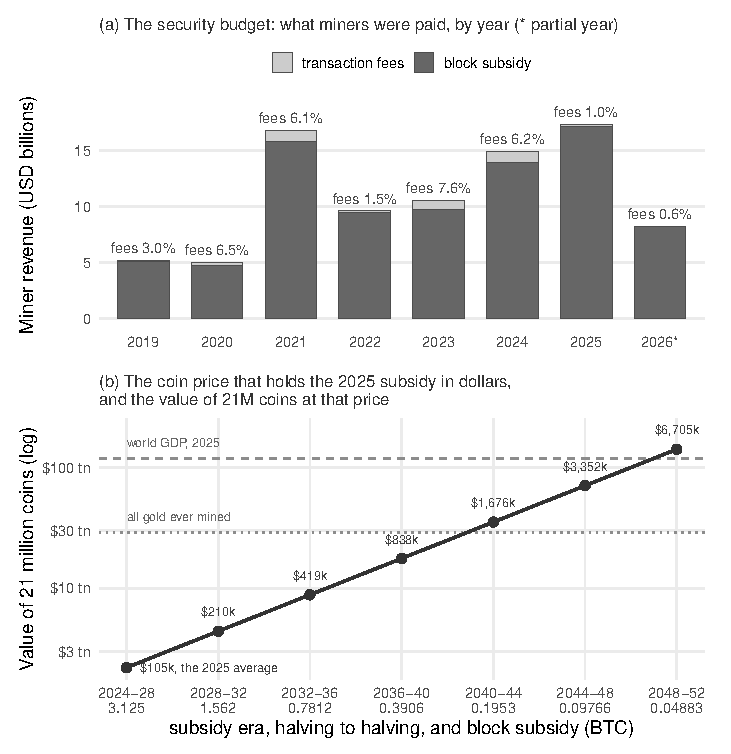
\includegraphics[width=\textwidth]{images/ch10_security_budget}
  \caption{(a)~The security budget by year: block subsidy and transaction fees paid to miners, in dollars, with the fee share. (b)~The price of one bitcoin that would hold the 2025 subsidy of \$17.2~billion constant in dollars through each coming halving, and the market value of 21~million coins at that price, against the value of all gold ever mined and a year of world output. Prices in the labels are per coin. Sources: miner revenue and fees, blockchain.com (daily, summed by year); world GDP, World Bank (2025); gold, World Gold Council (end-Q2 2026).} % fig-src: analysis/figures/fig_ch10_security_budget.R on analysis/data/ch10_security_budget_annual.csv and ch10_subsidy_schedule.csv (ch10_subsidy_arithmetic.R)
  \label{fig:outlook-budget}
\end{figure}

Table~\ref{tab:outlook-halving} does the sum. Hold the 2025 subsidy at its dollar value, \$17.2~billion a year, and ask what price each epoch's coins would have to fetch. The current epoch mints 164,250 coins a year, so the price is about \$105,000; the epoch that begins in 2028 mints half as many, so \$210,000; then \$419,000, \$838,000, \$1.7~million in 2040, \$3.4~million in 2044 and \$6.7~million in 2048. Multiply by 21~million coins. In 2040 the network would be worth \$35~trillion, more than every ounce of gold ever mined, which the World Gold Council valued at \$29~trillion in mid-2026. In 2048 it would be worth \$141~trillion, more than a year of the world's entire output, which the World Bank put at \$118~trillion for 2025 \autocite{worldbank2025gdp,wgc2026gold}. The gold comparison sets a stock against a stock; the output comparison sets a stock against a flow and is offered for scale, not as a limit, and both are in today's dollars against today's gold and today's output. % src: ch10_subsidy_arithmetic.R console (price for constant 2025 subsidy: 104,765 / 209,530 / 419,060 / 838,120 / 1,676,240 / 3,352,480 / 6,704,960; caps 2.2 / 4.4 / 8.8 / 17.6 / 35.2 / 70.4 / 140.8 $tn; gold $29.0 tn; GDP $118.35 tn)
The price of bitcoin can grow exponentially and has; what it cannot do is double every four years without end. Nor does a growing world economy rescue the path: output grew about 5~percent a year in dollars over 2023 to 2025, and on a price growing at that rate the dollar subsidy still falls by a factor of 0.61 every epoch, since a half times 1.05 to the fourth power is 0.61. With output growing at that rate the crossing moves from 2048 to about 2056, two halvings later, and does not disappear. % src: ch10_subsidy_arithmetic.R console (World Bank 2023 $107.35 tn to 2025 $118.35 tn = 5.0% a year; 0.5 x 1.05^4 = 0.61; constant-subsidy value of 21M coins exceeds growing world output from the 2056 epoch, 1.06x, against 2048 at fixed 2025 output)
No reader needs to decide what bitcoin is worth to see where this ends. A dollar subsidy held constant by price requires bitcoin to pass all the gold in the world within four halvings and a year of the world's output within six, or eight if the world keeps growing. My reading is that holding the subsidy constant in dollar terms becomes increasingly implausible beyond the 2030s under these assumptions.

\begin{table}[htb]
  \centering
  \scriptsize
  \setlength{\tabcolsep}{2pt}
  \begin{tabular}{lrrrrr}
    \hline
    \textbf{Epoch} & \textbf{Subsidy} & \textbf{Coins} & \textbf{Price to hold} & \textbf{21M coins} & \textbf{Fees to hold} \\
    from & BTC/block & per year & 2025's \$ & gold / GDP & 2025's \$, \$bn \\
    \hline
    Apr 2024 & 3.125 & 164,250 & 104,765 & 0.08 / 0.02 & 4.0 \\
    Apr 2028 & 1.5625 & 82,125 & 209,530 & 0.15 / 0.04 & 10.7 \\
    Apr 2032 & 0.78125 & 41,062 & 419,060 & 0.30 / 0.07 & 14.0 \\
    Apr 2036 & 0.39063 & 20,531 & 838,120 & 0.61 / 0.15 & 15.7 \\
    Apr 2040 & 0.19531 & 10,266 & 1,676,240 & 1.21 / 0.30 & 16.6 \\
    Apr 2044 & 0.09766 & 5,133 & 3,352,480 & 2.43 / 0.59 & 17.0 \\
    Apr 2048 & 0.04883 & 2,566 & 6,704,960 & 4.86 / 1.19 & 17.2 \\
    \hline
  \end{tabular}
  \caption{The halving schedule against a price path. Coins per year are 52,560 blocks times the subsidy; ``price to hold 2025's dollars'' is the 2025 subsidy revenue of \$17.2~billion divided by the epoch's coins; the next column values 21~million coins at that price against all gold ever mined (\$29.0~trillion, World Gold Council, end of the second quarter of 2026) and world GDP (\$118.35~trillion, World Bank, 2025). The last column is the fee revenue that would hold the 2025 security budget of \$17.4~billion with the price fixed at \$81,273, the price on September 4, 2026, at which the subsidy itself is worth \$13.4~billion a year in the current epoch, \$6.7~billion from 2028 and \$3.3~billion from 2032; 2025 fees were \$0.18~billion. Both bases run slightly high: 2025 ran about 53,100 blocks as hashrate grew, 1~percent more, and the revenue series behind the \$17.2~billion runs 2~percent above the coins issued times each day's price, so on 2025's own coins and prices the fourth and fifth columns would be about 3~percent lower, from \$101,700, every crossing in the same epoch, and each fee in the last column \$0.3~billion lower. Epoch dates after 2024 assume ten-minute blocks; subsidies are rounded to five decimals where needed.} % tab-src: analysis/data/ch10_subsidy_schedule.csv, written by analysis/checks/ch10_subsidy_arithmetic.R; basis lines of its console (2025: 53,082 blocks, 165,881 coins, 1.0% over 52,560; revenue-series subsidy $17.21 bn is 2.0% above coins issued x daily price, $16.87 bn; current-epoch price $101,705, 2.9% below $104,765; crossings on that basis gold 2040 at 1.18x, 2025 GDP 2048 at 1.15x, growing GDP 2056 at 1.03x; budget $17.05 bn, $0.34 bn below $17.38 bn, current-epoch fee $3.70 bn against $4.03 bn)
  \label{tab:outlook-halving}
\end{table}

The record so far has one epoch on each side of the doubling the table requires. Between the 2020 and 2024 halvings the price rose 7.3-fold, more than enough to grow the dollar subsidy through a halving; in the two years and four months since the 2024 halving it has risen 27~percent, less than the halving took away. % src: ch10_subsidy_arithmetic.R console (price $8,754 on 2020-05-11; $63,824 on 2024-04-20; $81,273 on 2026-09-04)
The subsidy in dollars fell from \$15.8~billion in 2021 to \$9.5~billion in 2022, and stood at \$17.2~billion in 2025 with half the coins per block. % src: ch10_subsidy_arithmetic.R console (subsidy revenue 2021 15.8, 2022 9.5, 2023 9.8, 2025 17.2 USD bn)
Hashprice tells the same story from the miner's chair: it fell six-fold from 2021 to 2025 while the price of bitcoin roughly doubled, because the coins per block halved once and the hashrate competing for them grew about six-fold. % src: chapter 4 and chapter 9 (hashprice $0.310 to $0.051 per TH-day); analysis/data/hashprice_daily_2021on.csv: mean hashrate 145 EH/s in 2021, 928 EH/s in 2025; mean price $47,386 in 2021, $101,682 in 2025 = 2.15x

So when does the subsidy become too low to finance the business? Mining is never too unprofitable to exist, because difficulty adjusts: when the dollar subsidy falls, the least efficient machines leave, hashrate falls, and the miners who remain earn the same subsidy over fewer hashes until the business clears again. What falls is not the existence of mining but its size, and its size is the network's security. If the price stays where it is, the dollar subsidy is \$6.7~billion a year from 2028, \$3.3~billion from 2032 and \$1.7~billion from 2036, and the hashrate the network can pay for shrinks with it, by whatever share machine efficiency does not recover. For fees to hold the 2025 budget instead, users of block space would have to pay \$10.7~billion a year from 2028 and \$14~billion from 2032, against \$0.18~billion in 2025: sixty to eighty times 2025's fee revenue. % src: ch10_subsidy_arithmetic.R console (subsidy at $81,273: 6.67 / 3.34 / 1.67 $bn; fees needed 10.71 / 14.05 $bn vs 0.175 $bn in 2025)
No year in the record of Figure~\ref{fig:outlook-budget}(a) has seen fees on that scale, which leaves the question of who else might pay.

\section{Who Pays for Security When the Subsidy Is Gone}
\label{sec:outlook-payers}

Three parties could fund the hashes that the subsidy no longer does. What follows is my reading of each, on a record that thins from the first to the third.

The first is the grid, and Section~\ref{sec:outlook-cheaper} is the offer on the table. As hashprice falls, the grid's payments for flexibility grow from a tenth of a mine's revenue toward the whole of its margin, and a site that could not cover its power and grid costs on mining alone covers them with its switch. This is real, and it is the subject of this book, but it has a ceiling that the same table shows. The grid pays for the hours a mine is off. At a quarter of the 2025 hashprice the flexible site cleared its power and grid charges by \$4~million where the never-pausing one fell \$11~million short, but it did so with the S19j~Pro off 69~percent of the year and the S21~XP 40~percent, and a machine that is off produces no hashes. % src: ch10_hashprice_sensitivity.R console (25% row: off 68.9% / 39.6%)
The grid can keep a fleet in business; it cannot keep it hashing. The size of the grid's contribution says the same thing from the other side. Chapter~9's site earned about \$101,000 of flexibility per megawatt-year in 2025; on the roughly 4,600~MW of mining demand ERCOT carried at its 2025 peak, that is about \$0.5~billion a year against a security budget of \$17.4~billion, under 3~percent, and even at a quarter of the 2025 hashprice, \$227,000 per megawatt-year, it is \$1.0~billion. Most of it is cost avoided rather than cash received: the strike and the power target lower the power bill, the window removes a charge, and only reserves put money in. % src: ch10_hashprice_sensitivity.R console, grid sizing ($100,920 and $227,393 per MW-yr x 4,600 MW = $0.46 bn and $1.05 bn, $1.046 bn unrounded, so $1.0 billion; $101,270 and $229,829, printed $230,000 and $1.1 billion, until 2026-10-03, when the ledgers booked distribution at $0.50 per MWh consumed; the older $100,604 / $228,928 in this comment did not reproduce and was corrected 2026-09-20); chapter 7 opening (potomac2026somercot pp. i, 31, ~4,600 MW, the 2025 peak of aggregate mining demand; both the per-MW-year value, flex value / 67.13 MW of site capacity, and the 4,600 MW are capacity bases); chapter 9 fig:stack-shape (reserves the only cash segment, 2022 and 2024 of the planned site)
This is still the most important development in the economics of mining since the industrial ASIC, and it is not a substitute for the subsidy.

The second party is the users of block space, through fees, and the arithmetic above says what they would have to pay.

The third party is the holders, and this is the chapter's third sum. A holder of bitcoin benefits from every hash whether or not they paid for it, which is the shape of a public good: everyone benefits, nobody is billed. Such a good can be paid for when one beneficiary is large enough that the benefit to itself covers the cost. Holders already pay, through dilution, about \$172~million a year for each percent of the supply they hold (Section~\ref{sec:outlook-budget}); the question the schedule forces is whether they will pay explicitly when issuance no longer collects it for them, the way the owner of a vault pays the guards. The record has two cases, and only one of them touches mining. Tether, the issuer of the largest dollar stablecoin, has invested in generation and mining since 2023, from a 241~MW renewable park in El Salvador to a proposal in April 2026 to vote its shares for mergers of Twenty One Capital with the bitcoin financial services company Strike and with Elektron Energy, a large mining platform; by August, Twenty One had dropped Strike and had no binding agreement with Elektron \autocite{tether2023volcano,tether2026twentyone,xxi2026q2}. % src: tether2023volcano (Volcano Energy, 241 MW, Metapan); tether2026twentyone (April 29, 2026, re-read 2026-09-27: Tether Investments "intends to vote its shares in favor of a proposed merger between XXI and Strike", and of the combined entities with Elektron Energy, "a large-scale Bitcoin mining platform"); xxi2026q2 (Form 10-Q filed 2026-08-11: "no longer pursuing the acquisition of Strike", announced July 21, 2026; Risk Factors: "Strike, a leading Bitcoin financial services company", re-read 2026-09-27; "no binding commitments or agreements with respect to the acquisition of Elektron"); the registrant's name is Twenty One Capital, Inc., with no hyphen
The United States established a Strategic Bitcoin Reserve by executive order in March 2025, capitalized with forfeited coins that ``shall not be sold,'' and directed its Treasury and Commerce departments to find budget-neutral ways of acquiring more; the order, which says nothing about mining, stood unamended in September 2026 \autocite{whitehouse2025sbr}. % src: whitehouse2025sbr sec. 3(a), 3(c), re-read 2026-09-27 (no "mining", "miner" or "mine" in the text); Federal Register API, 2026-09-27: EO 14233 (document 2025-03992) has no disposition or executive-order notes, and a term search for "Strategic Bitcoin Reserve" returns only the order itself
Neither is a central bank buying hashrate. What the record points at is a structure rather than an event: a large holder that funds mining is paying for the security of its own balance sheet, and a large holder that funds mining next to a grid that pays for the mine's flexibility is splitting the bill with the grid. The miner sells the switch to the grid and the hashes to the holder. Whether treasuries, sovereign or corporate, come to see the security budget as a cost of holding the asset is the open question. The arithmetic of Section~\ref{sec:outlook-halving} forces it within two halvings, and the parties with the most to lose from leaving it open are the ones with the most coins.

\section{What the Book Adds Up To}
\label{sec:outlook-close}

Chapter~2 described a grid as a huge, humming engine that must be balanced every second, and a mine as a load that can be balanced against it. Eight chapters later the claim can be stated exactly. A mine holds one asset the grid cannot buy from a gas plant or a battery: the freedom to change what it draws inside a quarter-hour and to hold the change for as long as the grid needs, an hour or a February week, at a cost the machines were built to bear. Chapter~4 priced the threshold at which a miner exercises that freedom, Chapter~5 built the loop that exercises it, and Chapter~6 found the contracts that leave the switch in the miner's hand. Chapters~7 and~8 found the markets and the tariffs that pay for it. Chapter~9 found that the whole, set as an operator could have set it in advance, was worth 9.0, 8.0 and 15.8~percent of a site's margin after power and grid charges in 2022, 2024 and 2025 and 23.0 and 29.5~percent of it in 2021 and 2023, where hindsight would have made the storm year 52.6~percent, and that a fence with a cheap price is worth having only when it is firm. % src: chapter 2 opening (humming engine; balanced every second); chapter 9 sec:stack-rule; analysis/checks/ch9_optimal_stack.R console, re-run 2026-10-03: PLANNED lines, flexibility over never pausing (23.0% in 2021, 9.0% in 2022, 29.5% in 2023, 8.0% in 2024, 15.8% in 2025), and the 2021 HINDSIGHT CEILING line (52.6%; 52.7% until 2026-10-03, when the ledgers booked distribution at $0.50 per MWh consumed); the same shares are plan_flex / never_total and hind_flex / never_total in analysis/data/ch9_optimal_stack.csv

This chapter added the direction of travel. As hashprice falls, flexibility becomes a larger share of mining revenue in the modeled cases. Halvings push in that direction; price, fees and network hashrate decide how far it goes. The grid a mine joins is one that has asked for flexible load in so many words and is filling up with firm compute that will need a flexible layer beside it. And, on my reading of the second sum, the subsidy that has paid for the network's security so far cannot be held in dollars past the 2030s without bitcoin passing all the gold in the world, which, if the price stays near where it is, puts the question of who pays for the hashes on the table within two halvings. The grid is one of the answers, and this book has spent its length measuring it. It is not the whole answer.

Three predictions, then, in the first person and dated to the April 2028 halving, each tied to a table this book's repository will recompute. I expect the S21 generation to be running the S19j~Pro's game by then, with the older fleet's strike under the mean price in most zones (Table~\ref{tab:outlook-sensitivity}); the peak layer gone for new large loads and the payment for flexibility settled on the five-minute price (Section~\ref{sec:outlook-grid}); and the fee share of the security budget still in single digits (Figure~\ref{fig:outlook-budget}). What would prove me wrong: a fee market that holds a tenth of the budget for a full year; a price path above the doubling staircase of Table~\ref{tab:outlook-halving} for two epochs running; a final 12CP rule that keeps a peak game for new large loads; or a first full RTC+B year in which reserve prices recover. On this reading each halving enlarges the grid resource: every epoch turns each fleet into the previous fleet's marginal machine, whose flexibility is the largest share of what it earns.

That is why the book has the title it has. Bitcoin mining is a grid resource because its flexibility is the product, and the product is real: measured on public data, paid for by a market that did not design it, and, on the arithmetic of Table~\ref{tab:outlook-sensitivity}, a larger share of what a mine earns the further hashprice falls. What the bitcoiner takes from the grid's side of the ledger is that the less a hash is worth, the more of what the machine earns comes from answering the grid. % src: tab:outlook-sensitivity, flexibility as a share of mining revenue 9.4 / 13.8 / 26.1 / 47.8 / 84.3% at 100 / 75 / 50 / 35 / 25% of the 2025 hashprice, 2025 prices held (analysis/data/ch10_hashprice_sensitivity.csv, written by analysis/checks/ch10_hashprice_sensitivity.R), the claim's only support; chapter 9's ledger shares (planned 23.0 / 9.0 / 29.5 / 8.0 / 15.8% of profit, 2021-2025) move with scarcity, not in a trend, so they are not cited for it
What the grid engineer takes from the miner's side is that the load that follows the price best is the one whose economics force it to. Neither side needs to believe in the other's asset for the arrangement to work. They only need to agree on the price of a quarter-hour, and that, in Texas, they already do.
